This section gives a high-level overview of the functional blocks of the tachometer. Figure~\ref{fig:block} shows the tachometer block diagram.


\begin{figure}[H]
    \centering
    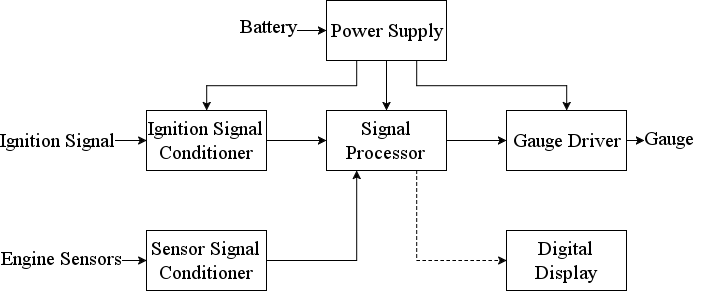
\includegraphics[width=\textwidth]{blocks}
    \caption{Tachometer block diagram}
    \label{fig:block}
\end{figure}

The system works as follows: the power supply is a switching DC-DC converter that steps the nominal 12V of the battery down to a regulated 5V to power the project. Additionally, a linear DC-DC converter steps the battery voltage down to 10V for the gauge driver circuitry, discussed later. The ignition signal conditioner block filters the ignition signal to produce a 0V to 5V square wave for the signal processor. The ignition signal conditioner protects the rest of the system from the high voltages of the ignition system. The sensor signal conditioner steps 12V signals from the temperature, pressure, and voltage sensors down to 5V signals. Signals from the the ignition and sensor conditioners go to the signal processor, which is responsible for controlling the gauge driver and digital display. The gauge driver amplifies the signal from the signal processor to drive the gauge to the proper position. The signal processor can be calibrated upon installation, allowing the tachometer to be adjusted to gauge variations. The digital display is a detachable LCD screen which is capable of displaying the engine RPM as well as the other specified inputs.


\subsection{Power Supply}
The power supply, a switching DC-DC converter, steps the 12V battery voltage down to 5V positive voltage rail of the tachometer. A switching DC-DC converter is more efficient than a linear regulator and thus dissipates less heat. The DC-DC converter uses a TI simple switcher integrated circuit, which simplifies the design and construction process. Using a simple switcher means no need to select a transistor or design a bootstrap circuit, a complicated process with a conventional DC-DC converter. It also has a built in feedback network, which is able to compensate for variations in the input voltage. 


\subsection{Ignition Signal Conditioner}
The ignition signal conditioner (ISC) converts the ignition signal from the engine into a digital signal for the signal processor. As the ignition signal is generated by the engine's ignition coil, a significant amount of electrical noise is present with the signal. Voltage spikes in excess of 100V are also present, which would damage the signal processor if not properly handled. To protect the rest of the tachometer circuitry from these voltage spikes, the ISC must prevent the ignition signal from exceeding the positive rail voltage or dipping below the reference rail voltage (0V).

To increase the signal processor's ability to reliably measure the ignition signal frequency, the ISC must also filter out the high frequency noise caused by the ignition coil. A low pass filter, operational amplifier buffer, and a comparator accomplish the task of generating a low-noise square wave which is then fed to the signal processor.

\subsection{Gauge Driver}

The gauge driver runs the physical tachometer gauge. The gauge operates by controlling the voltages on the three input wires to change the magnetic field in the gauge. The gauge driver amplifies the signal from the signal processor to drive the gauge.

\subsection{Sensor Signal Conditioner}

The sensors in the engine operate on the logic level of the battery ($\sim$12V). To allow the signal processor to measure the sensor signals, they must first be reduced to a 5V logic level. The engine sensors consist of heat-varying, and pressure controlled resistors for engine temperature and oil pressure, respectively. The gauges in the dashboard of the boat drive a current through the resistive sensors and measure their voltages. So as not to affect the sensor readings with the measurement circuitry, the signal conditioner uses a high input impedance resistive voltage divider followed by an operational amplifier unity gain buffer. The output of this stage is a 0V to 5V direct current signal.

\subsection{Digital Display}

The digital display lets the user see a readout of the engine RPM and engine sensors. The display can safely be hot swapped when the tachometer is in operation. When the display is connected, a signal is sent to the signal processor to indicate its presence. The display is then initialized to output engine sensor information.

\subsection{Signal Processor}
The signal processor takes input signals and produces output signals that ultimately become human readable. First, the signal processor receives the conditioned tachometer signal and calculates its frequency. An algorithm finds engine RPM from the input and produces an output signal to run the gauge driver.

Next, an analog to digital converter (ADC) converts the engine sensor inputs to a digital value. An ADC calibration algorithm converts these input values into output values for pressure, temperature, and battery voltage. Finally the signal processor sends the engine RPM and human readable sensor information to the digital display and gauge driver.